\chapter{Data Extraction and Processing}
\label{scraping}

This chapter details the methodology for extracting, organising and processing data from digital match reports made available by the \textit{Confederação Brasileira de Futebol} (CBF).

The CBF maintains, since 2013, a repository with open access to match reports in PDF format.
These reports can be accessed through CBF's website (\url{https://www.cbf.com.br}) or using the following URL pattern: \url{https://conteudo.cbf.com.br/sumulas/{year}/{championship_id}{game_id}se.pdf}.
The championship identifiers are shown in Table~\ref{tab:championship_id}.
The game ID is an incremental integer, one for each game and defined before the start of the championship, which may result in gaps when a game is postponed during the season.

\begin{table}[htbp]
    \centering
    \begin{tabular}{ccc}
        \toprule
        Championship ID & Championship Name                      & Details \\
        \midrule
        142             & \textit{Campeonato Brasileiro Série A} & Brazilian First Division \\
        242             & \textit{Campeonato Brasileiro Série B} & Brazilian Second Division \\
        342             & \textit{Campeonato Brasileiro Série C} & Brazilian Third Division \\
        542             & \textit{Campeonato Brasileiro Série D} & Brazilian Fourth Division \\
        424             & \textit{Copa do Brasil}                & National Cup \\
        \bottomrule
    \end{tabular}
    \caption{
        \textbf{Championship ID pattern on CBF's website}.
        The IDs used for accessing match reports on CBF's website.
    }
    \label{tab:championship_id}
\end{table}

\section{Structure of CBF PDF Reports}
\label{sec:report_structure}

Figure~\ref{fig:report_example} shows an example of a match report from the 2013 season between CR Vasco da Gama and Associação Portuguesa de Desportos.
This example illustrates how the report is structured and helps understand how the principal information can be extracted.

\begin{figure}[htbp]
    \centering
    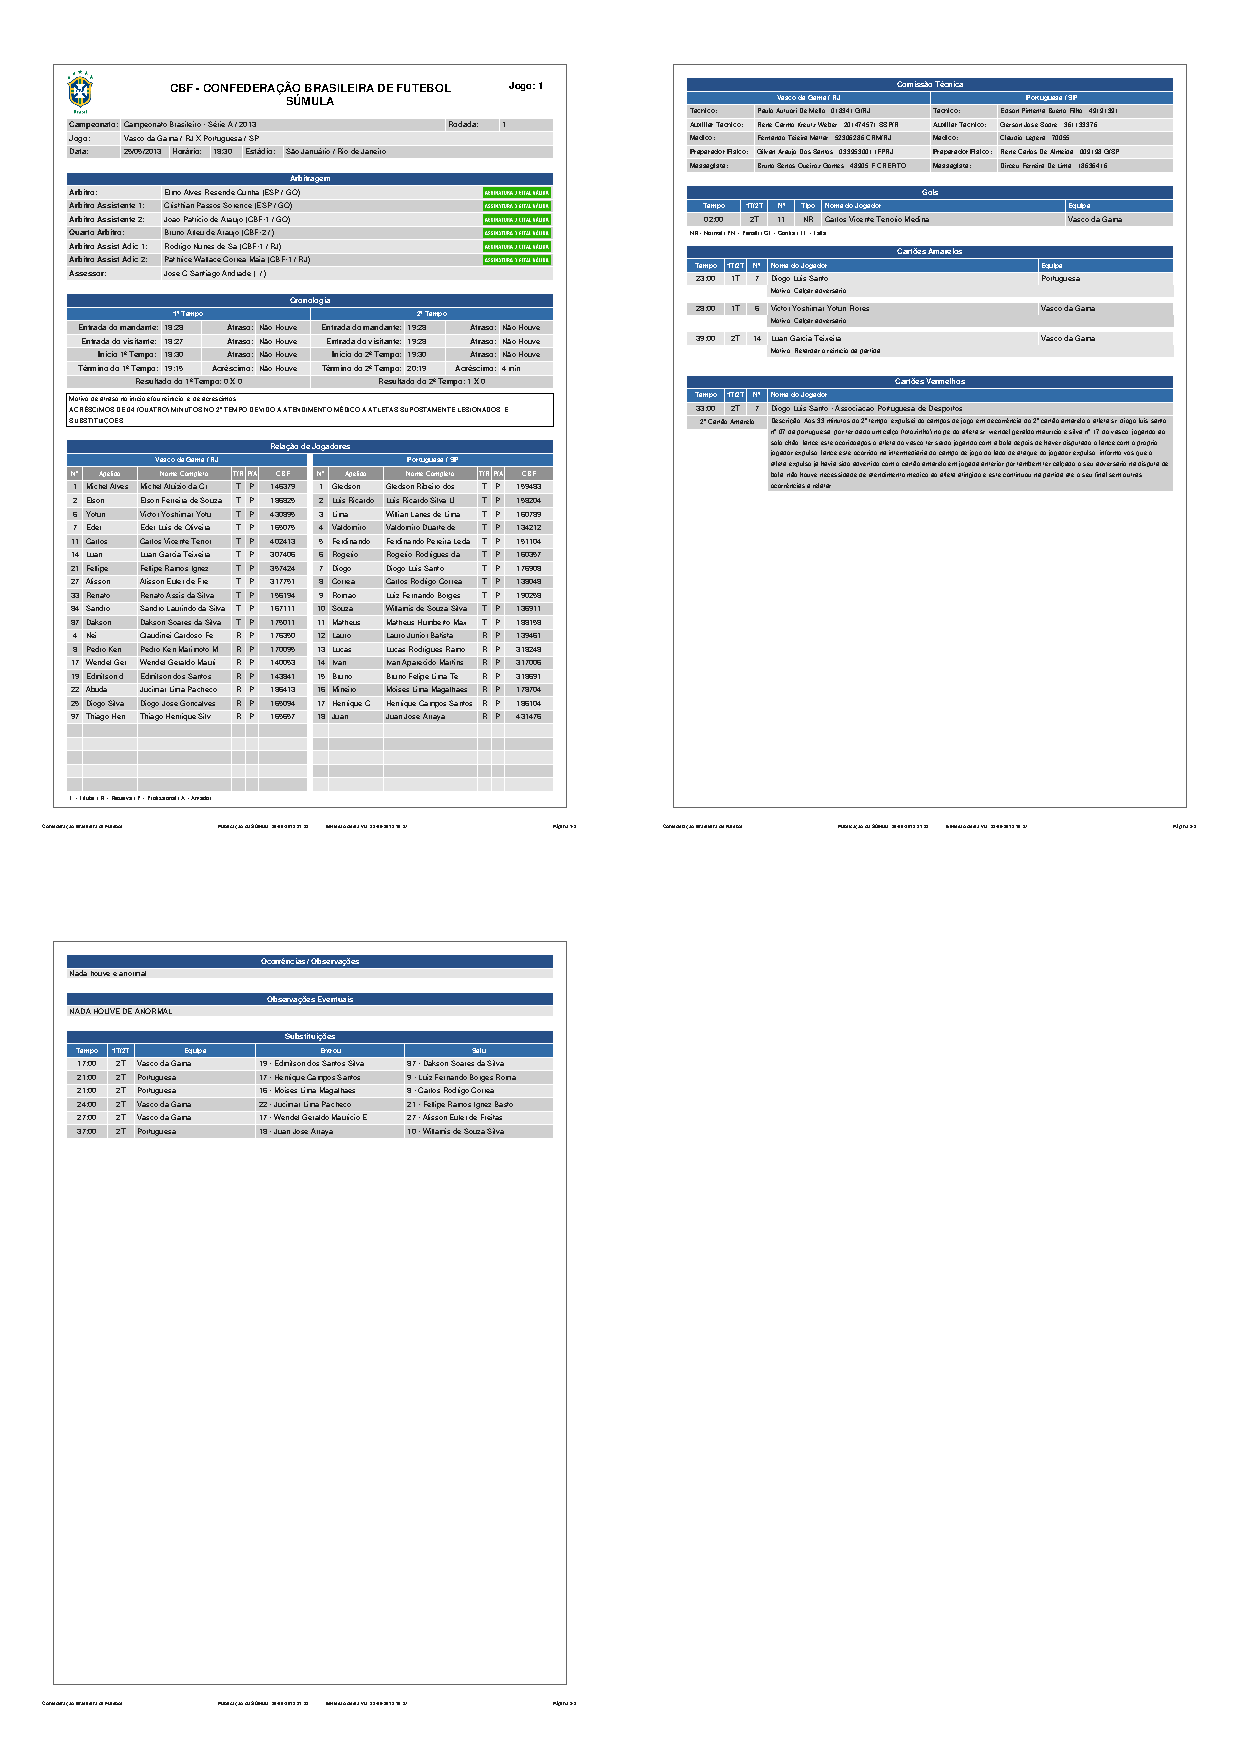
\includegraphics[width=0.9\textwidth]{figures/report.pdf}
    \caption{
        \textbf{Example of a CBF match report}.
        Example report from a match between CR Vasco da Gama and Associação Portuguesa de Desportos, which took place on May 25th, 2013, for the first round of the Brazilian First Division (\textit{Série A}).
    }
    \label{fig:report_example}
\end{figure}

The report begins with a header containing match details: championship, round, game, date, time, and stadium.
Then, we have the referee information, followed by the chronological details of the game.

Next, we have the player line-up relation as two tables, one for each club.
For each player, the table includes their jersey number, nickname, and full name.
Players in the starting line-up are marked with a ``T'', while substitutes are marked with a ``R''.
The table also indicates whether each player is professional (P) or amateur (A).
Each player is identified by their unique CBF id, which we use internally throughout our data extraction and processing workflow instead of player names, since names are more sensitive to encoding issues and may have inconsistent accentuation across reports.
Following the players' relation we have information on the coaching and medical staff.

After the team information, the report contains data on the events that occurred during the match.
This section starts with the goals scored during the match.
The report saves this information on two columns for time because in Brazil the game is divided and counted in two periods with 45 minutes each.
In this sense, unlike other countries, the minute 65 of a game is assigned as 20 minutes of the second period.
For each goal, the table includes when it was scored (minute and period), the scorer's jersey number and name, the type of goal, which can be open-play (NR), penalty (PN), own goal (CT), or free kick (FT), and the club for which the goal counts.

Yellow and red card data is found right after the goal data.
The first section is related to yellow cards, while the second is to red cards.
The organization of these sections follows the same structure as the goals table, except that the goal type field is not applicable.
For each card, the table includes when it was shown (minute and period), the player's jersey number and name.
An extra field, right below the player's name, indicates the reason for the card, though this information is not extracted in our retrieval process.

After these sections, we have substitution information.
This section is also organized as a table.
For each substitution, the table includes when it was made (minute and period), which club made the substitution, and the jersey number and full name of both the player entering and the player exiting the field.

At the end of the report, we have two sections for any occurrence or observation that the referees' team thinks is relevant.


\section{Data Retrieval Process}
\label{sec:retrieval}

The data retrieval process begins with extracting the PDF reports from CBF's website.
We use the Python package \textsc{requests} \cite{requests}, passing the URL pattern described in Section~\ref{sec:report_structure} as an argument.
After making the request, we validate the response and, if valid, save the PDF file to disk.
To avoid overwhelming CBF's server, once a report is successfully saved, we do not make additional requests for that same report.

With the saved PDF, we open it using \textsc{PdfReader} from the \textsc{PyPDF2} package \cite{pypdf2} and extract all text content to a CSV file, which is then saved to disk.
The parsing process is implemented in Python using the \textsc{re} package \cite{re} for regular expression matching to extract and parse the data from the CSV files, saving the structured information into JSON files.

From the file header, we extract the clubs' names and the final match result.
For both clubs in the game, we collect information about all players who participated in that match, including their jersey number, nickname and full name, starting condition (in the line-up or on the bench), professional status, the player's CBF code, and the club represented by the player in that game.

After extracting player information, we collect data on goals scored in the match.
For each goal, we save the moment (minute and period), the goal type (open-play, penalty, free kick, or own goal), the jersey number and name of the scorer, and the club for which the goal was scored.

We also extract information about substitutions that occurred during the game.
For each substitution, we save the moment of the change, the club that made the substitution, and the jersey number and name of both the player who entered and the player who exited.

Finally, we record information about yellow and red cards.
This data is saved with the same structure as goals, except for the goal type field.
An important note is that in this process, each half of the game is clipped to 45 minutes.
Therefore, all events that occurred during injury time are recorded as events at minute 45 of the corresponding period.

\begin{figure}[htbp]
    \centering
    \begin{tikzpicture}[
        node distance=0.9cm,
        >=Latex,
        thick,
        process/.style={
            draw,
            rounded corners,
            minimum width=4cm,
            minimum height=1cm,
            align=center,
            font=\small,
            fill=blue!15
        },
        save/.style={
            draw,
            rounded corners,
            minimum width=4cm,
            minimum height=1cm,
            align=center,
            font=\small,
            fill=cyan!15
        },
        decision/.style={
            diamond,
            aspect=2.2,
            draw,
            align=center,
            inner sep=1pt,
            fill=yellow!15,
            font=\small
        },
        startstop/.style={
            draw,
            rounded corners,
            minimum width=4cm,
            minimum height=1cm,
            align=center,
            font=\small,
            fill=red!15
        },
        skip/.style={
            draw,
            rounded corners,
            minimum width=4cm,
            minimum height=1cm,
            align=center,
            font=\small,
            fill=gray!15
        }
    ]
        % Main vertical flow
        \node[startstop] (start) {Start};
        \node[process, below=of start] (request) {Request PDF\\from CBF's site};
        \node[decision, below=of request] (valid) {Valid?};
        \node[save, below=of valid] (savepdf) {Save PDF};
        \node[process, below=of savepdf] (extract) {Extract text\\(PyPDF2)};
        \node[save, below=of extract] (savecsv) {Save to CSV};
        \node[process, below=of savecsv] (parse) {Parse with\\regex};
        \node[process, below=of parse] (extractdata) {Extract data};
        \node[save, below=of extractdata] (savejson) {Save to JSON};
        \node[decision, below=of savejson] (more) {More?};
        \node[startstop, below=of more] (end) {End};

        % Side branch
        \node[skip, right=2cm of valid, text width=4cm] (skip) {Skip};

        % Arrows
        \draw[->] (start) -- (request);
        \draw[->] (request) -- (valid);
        \draw[->] (valid) -- node[left] {Yes} (savepdf);
        \draw[->] (valid.east) -- node[above] {No} (skip.west);
        \draw[->] (savepdf) -- (extract);
        \draw[->] (extract) -- (savecsv);
        \draw[->] (savecsv) -- (parse);
        \draw[->] (parse) -- (extractdata);
        \draw[->] (extractdata) -- (savejson);
        \draw[->] (savejson) -- (more);
        \draw[->] (more) -- node[left] {No} (end);
        \draw[->, bend left=40] (more.west) to node[left] {Yes} (request.west);
        \draw[->] (skip) |- (more);
    \end{tikzpicture}
    \caption{
        \textbf{Data extraction workflow}.
        Overview of the extraction process: first extracting the reports from CBF's website, then processing the information through PDF to CSV conversion and JSON parsing.
    }
    \label{fig:extraction_flowchart}
\end{figure}


\section{Data Treatment and Normalization}
\label{sec:data_treatment}

As discussed in the previous section, most of the data registered in the reports concerns a player's jersey number and name.
This poses two problems: first, some clubs adopt a variable jersey number distribution during the season, where players in the starting line-up always have numbers from 1 to 11.
Secondly, using player names can be problematic because we have both the player's nickname and ``full name'', but the full name is often incomplete or truncated.
To address these issues, we convert all player references to CBF's unique ID system.
During the data extraction process, we substitute the player's name and jersey number with their personal CBF ID, ensuring consistent identification across matches and seasons.

Furthermore, our data processing workflow segments each game using all player substitutions and red cards to create temporal segments.
For each game, we generate ``sub-games'', each representing a period during which the same set of players was on the pitch, bounded by substitutions or red card events.
The final result is a JSON file with all games structured as shown in Figure~\ref{fig:json_structure}.
\begin{center}
    \lstset{style=json}
    \begin{lstlisting}
{
    "001": {
        "Summary": {
            "Home": "Vasco da Gama / RJ",
            "Away": "Portuguesa / SP",
            "Result": "1 X 0",
            "Date": "25/05/2013",
            "Time": "18:30",
            "Stadium": "São Januário / Rio de Janeiro"
        },
        "0": {
            "Home": {
                "Squad": ["146379", "186825", "430895", "165075", "402413", "307406",
                          "357424", "317751", "156194", "167111", "175011"],
                "Cards": [[[28, False], "430895"]],
                "Goals": [[[47, False], "402413"]]
            },
            "Away": {
                "Squad": ["159483", "158204", "160789", "134212", "151104", "160357",
                          "176908", "138048", "190258", "136911", "188158"],
                "Cards": [[[23, False], "176908"]],
                "Goals": []
            },
            "Time": 62
        },
        "1": {
            "Home": {
                "Squad": ["146379", "186825", "430895", "165075", "402413", "307406",
                          "357424", "317751", "156194", "167111", "143841"],
                "Cards": [],
                "Goals": []
            },
            "Away": {
                "Squad": ["159483", "158204", "160789", "134212", "151104", "160357",
                          "176908", "138048", "190258", "136911", "188158"],
                "Cards": [],
                "Goals": []
            },
            "Time": 4
        }
    }
}
    \end{lstlisting}
    \captionof{figure}{
        \textbf{Final JSON structure example}.
        Example of the game between CR Vasco da Gama and Associação Portuguesa de Desportos, showing two sub-games triggered by a substitution (CBF ID 175011 replaced by 143841) at the 62nd minute.
        The ``Summary'' field stores general metadata such as team names, final result, date/time, and venue.
    }
    \label{fig:json_structure}
\end{center}

The JSON structure can be interpreted as follows:
\begin{itemize}
    \item \texttt{"001"}: Represents the unique identifier for the match.
    \begin{itemize}
        \item \texttt{"Summary"}: Provides a summary of the match, including home team, away team, final result, date, time, and stadium.
        \item Other second-level keys (e.g., \texttt{"0"}, \texttt{"1"}, \texttt{"2"}, ...) represent different segments of the match.
        These segments are created whenever a substitution or red card occurs, even if the red card is shown to a reserve player.
        \begin{itemize}
            \item \texttt{"Home"} and \texttt{"Away"}: Information about each team during this segment.
            \begin{itemize}
                \item \texttt{"Squad"}: List of player CBF IDs for the team.
                \item \texttt{"Cards"}: List of cards received by team players.
                Each card is represented by an array where the first element is a tuple with the minute the card was shown and a boolean flag indicating whether it occurred during injury time of the current segment.
                The second element is the player's CBF ID.
                \item \texttt{"Goals"}: List of goals scored by the team, each represented by an array where the first element is a tuple with the minute the goal was scored and a boolean flag indicating whether it occurred during injury time.
                The second element is the scorer's CBF ID.
            \end{itemize}
            \item \texttt{"Time"}: Duration of this segment in minutes.
        \end{itemize}
    \end{itemize}
\end{itemize}

An important consideration in this process is that all reports are written manually, which means they may contain typos or mistakes.
When we identified anomalies that caused errors in the retrieval process, we manually corrected them.
However, this correction process was only performed for First Division (\textit{Série A}) matches.
Consequently, in lower divisions, we can expect more anomalies that were not treated, which may result in potentially inferior data quality for those competitions.


\section{Dataset Characterization}
\label{sec:dataset_stats}

The final dataset covers match reports from 2013 to 2025, encompassing the main Brazilian football competitions: the four divisions (\textit{Série A}, \textit{Série B}, \textit{Série C}, and \textit{Série D}) and the national cup (\textit{Copa do Brasil}).
In total, the dataset maps 16,800 unique players who played for 368 unique clubs across all competitions.
The complete dataset is publicly available on Zenodo \cite{michels_2026_dataset}.

Table~\ref{tab:total_games} shows the number of matches by season and championship, while Tables~\ref{tab:total_clubs} and~\ref{tab:total_players} show the distribution of clubs and players.
In these tables, each value corresponding to both a season and a championship represents the total number of games, unique players, or unique clubs for that championship during that season.
The ``Total unique'' columns in Tables~\ref{tab:total_clubs} and~\ref{tab:total_players} aggregate the players/clubs across all championships for the corresponding season, while the ``Total unique'' rows aggregate across all seasons for a given championship.
The final value in the bottom-right corner shows the total number of unique players/clubs in the entire dataset.

\begin{table}[htbp]
    \centering
    \begin{tabular}{ccccccc}
        \toprule
        Season & \textit{Série A} & \textit{Série B} & \textit{Série C} & \textit{Série D} & \textit{CdB} & Total games \\
        \midrule
        2013   & 380   & 380   & 213   & 188   & 156   & 1,317  \\
        2014   & 380   & 379   & 194   & 195   & 159   & 1,307  \\
        2015   & 380   & 380   & 194   & 190   & 158   & 1,302  \\
        2016   & 379   & 380   & 194   & 266   & 162   & 1,381  \\
        2017   & 380   & 380   & 193   & 266   & 120   & 1,339  \\
        2018   & 380   & 380   & 194   & 266   & 120   & 1,340  \\
        2019   & 380   & 379   & 194   & 266   & 120   & 1,339  \\
        2020   & 380   & 379   & 206   & 516   & 120   & 1,601  \\
        2021   & 380   & 380   & 206   & 518   & 122   & 1,606  \\
        2022   & 380   & 380   & 216   & 510   & 122   & 1,608  \\
        2023   & 380   & 380   & 216   & 510   & 122   & 1,608  \\
        2024   & 380   & 379   & 216   & 508   & 122   & 1,605  \\
        2025   & 380   & 375   & 214   & 507   & 121   & 1,597  \\
        \midrule
        Total  & 4,939 & 4,931 & 2,650 & 4,706 & 1,724 & 18,950 \\
        \bottomrule
    \end{tabular}
    \caption{
        \textbf{Total number of games by season and championship}.
        ``CdB'' stands for \textit{Copa do Brasil}, the national cup competition.
    }
    \label{tab:total_games}
\end{table}

\begin{table}[htbp]
    \centering
    \begin{tabular}{ccccccc}
        \toprule
        Season             & \textit{Série A} & \textit{Série B} & \textit{Série C} & \textit{Série D} & CdB & Total unique clubs \\
        \midrule
        2013               & 20      & 21      & 21      & 40      & 88  & 130                \\
        2014               & 20      & 20      & 20      & 41      & 87  & 132                \\
        2015               & 20      & 20      & 20      & 40      & 87  & 125                \\
        2016               & 20      & 20      & 20      & 68      & 86  & 147                \\
        2017               & 20      & 20      & 20      & 68      & 91  & 134                \\
        2018               & 20      & 20      & 20      & 69      & 91  & 138                \\
        2019               & 20      & 20      & 20      & 68      & 91  & 131                \\
        2020               & 20      & 20      & 20      & 68      & 91  & 136                \\
        2021               & 20      & 20      & 20      & 69      & 92  & 134                \\
        2022               & 20      & 20      & 20      & 64      & 92  & 129                \\
        2023               & 20      & 20      & 20      & 66      & 93  & 133                \\
        2024               & 20      & 20      & 20      & 65      & 92  & 137                \\
        2025               & 20      & 20      & 20      & 64      & 93  & 137                \\
        \midrule
        Total unique clubs & 37      & 66      & 83      & 297     & 294 & 368                \\
        \bottomrule
    \end{tabular}
    \caption{
        \textbf{Total number of clubs by season and championship}.
        ``CdB'' stands for \textit{Copa do Brasil}, the national cup competition.
    }
    \label{tab:total_clubs}
\end{table}

\begin{table}[htbp]
    \centering
    \begin{tabular}{ccccccc}
        \toprule
        Season               & \textit{Série A} & \textit{Série B} & \textit{Série C} & \textit{Série D} & \textit{CdB}  & Total unique players \\
        \midrule
        2013                 & 709     & 811     & 687     & 1,061    & 1,799 & 3,644                 \\
        2014                 & 736     & 833     & 650     & 1,043    & 1,872 & 3,671                 \\
        2015                 & 715     & 805     & 667     & 1,056    & 1,897 & 3,672                 \\
        2016                 & 722     & 775     & 666     & 1,603    & 1,847 & 4,012                 \\
        2017                 & 722     & 731     & 601     & 1,551    & 1,591 & 3,783                 \\
        2018                 & 720     & 740     & 584     & 1,563    & 1,605 & 3,745                 \\
        2019                 & 691     & 740     & 618     & 1,553    & 1,579 & 3,748                 \\
        2020                 & 733     & 791     & 690     & 2,032    & 1,695 & 4,381                 \\
        2021                 & 713     & 733     & 674     & 2,049    & 1,851 & 4,398                 \\
        2022                 & 747     & 796     & 685     & 2,037    & 1,835 & 4,322                 \\
        2023                 & 736     & 771     & 682     & 1,886    & 1,833 & 4,127                 \\
        2024                 & 709     & 756     & 674     & 1,965    & 1,817 & 4,231                 \\
        2025                 & 731     & 786     & 693     & 1,973    & 1,774 & 4,278                 \\
        \midrule
        Total unique players & 3,467    & 4,657    & 4,738    & 11,141   & 9,782 & 16,800                \\
        \bottomrule
    \end{tabular}
    \caption{
        \textbf{Total number of players by season and championship}.
        The totals do not correspond to simple sums because they count unique players across seasons.
    }
    \label{tab:total_players}
\end{table}

